\documentclass[12pt]{article}
\usepackage{graphicx}
\usepackage{epstopdf}
\usepackage{float}
\usepackage{commath}
\usepackage{textcomp}
\usepackage{amsmath}
\usepackage{caption}
\usepackage{subcaption}
\usepackage{float}
\usepackage{commath}

%
% Title.
\title{Digital Signal Processing 
   \\ Filter Design Assignment}

% Author


% begin the document.
\begin{document}


% make a title page.
\maketitle
\section{Assignment Details}
Student Name: \newline 
              Rachna Pawar\\
              Mohammad Shahbaz Alam\\
Filter Number: 46\\


\section{Filter - I: Bandpass Filter Design(Butterworth) }
\subsection{Un-normalized Discrete Time Filter Specifications}
Passband Tolerance = 0.15 (i.e 0.85-1.15)\\
Stopband Tolerance = 0.15 (i.e 0-0.15)\\
Analog Signal frequency range = 140 kHz\\
Sampling Frequency($f_s$) = 320 kHz\\
Transition band on either side of Passband = 2 kHz\\ 
Passband Nature : Monotonic\\
Stopband Nature : Monotonic\\\\
Assigned Filter Number = 46\\
q(46) = 4, r(46) = 6\\
$B_L(46)$ = 5 + 1.4*4 + 4*6 = 34.6 kHz\\
$B_H(46)$ = 34.6 + 10 = 44.6 kHz
\subsection{Normalized Digital Filter Specifications}
Sampling Frequency = 320 kHz\\
Therefore, normalized frequency can be calculated as,
\begin{equation}
    \omega = \frac{\Omega*2\pi}{\Omega_s}
\end{equation}
Making calculations as per above equation, the modified specifications are,
\\\\
Lower Passband Edge ($\omega_{p1}$) = 0.216$\pi$\\
Upper Passband Edge ($\omega_{p2}$) = 0.278$\pi$\\
Transition band on either side of Passband ($\omega_T$) = 0.0125$\pi$ 
\\Upper stopband Edge ($\omega_{s2}$) = 0.290$\pi$\\
Lower stopband Edge ($\omega_{s1}$) = 0.203$\pi$\\
Passband Nature : Monotonic\\
Stopband Nature : Monotonic\\
Passband Tolerance = 0.15 (i.e 0.85-1.00)\\
Stopband Tolerance = 0.15 (i.e 0-0.15)
\subsection{Equivalent Analog filter Specifications}
The analog filter specifications($\Omega$) can be determined using bilinear transformation on normalized specifications($\omega$) as,
\begin{equation}
    \Omega = tan(\frac{\omega}{2})
\end{equation}
Lower Passband Edge ($\Omega_{p1}$) = 0.352\\
Upper Passband Edge ($\Omega_{p2}$) = 0.466\\
Upper stopband Edge ($\Omega_{s2}$) = 0.489\\
Lower stopband Edge ($\Omega_{s1}$) = 0.330\\
\begin{equation}
    tan(\frac{0}{2}) = 0
\end{equation}
\begin{equation}
    tan(\frac{\pi}{2}) = \infty
\end{equation}
\subsection{Frequency Transformation for BPF to LPF conversion}
The frequency transformation employed for Band pass filter to equivalent low pass filter conversion,
\begin{equation}
    \Omega_L = \frac{\Omega^2-\Omega_o^2}{B*\Omega}
\end{equation}
where,\\ 
B = $\Omega_{p2}-\Omega_{p1}$ = 0.114\\
$\Omega_o^2$ = $\Omega_{p1}*\Omega_{p2}$ = 0.164\\

\subsection{Frequency transformed LPF Specifications}
\begin{equation}
    \Omega_L = \frac{\Omega^2-0.164}{0.114*\Omega}
\end{equation}
Lower Passband Edge ($\Omega_{p1}$) = -0.99\\
Upper Passband Edge ($\Omega_{p2}$) = 1.00\\
Upper stopband Edge ($\Omega_{s2}$) = 1.34\\
Lower stopband Edge ($\Omega_{s1}$) = -1.46\\\\

Passband Edge ($\Omega_{pl}$) = 1\\
Stopband Edge ($\Omega_{sl}$) = min(1.46,1.34) = 1.34\\
Passband and Stopband Tolerance = 0.15\\
Passband Nature = Monotonic\\
Stopband Nature = Monotonic

\subsection{Analog Lowpass Transfer Function}
The magnitude squared response of the butterworth filter in frequency domain,
\begin{equation}
    |H_{analog,LPF}(j\Omega)|^2 = \frac{K}{1 + (\frac{\Omega}{\Omega_c})^{2N}}
\end{equation}
where, K is the normalization constant.\\
Passband Tolerance($\delta_1$) = 0.15\\
Stopband Tolerance($\delta_2$) = 0.15\\
Defining,
\begin{equation}
    D_1 = \frac{1}{(1-\delta_1)^2}-1 = 0.384 
\end{equation}
\begin{equation}
    D_2 = \frac{1}{\delta_2^2}-1 = 43.44 
\end{equation}
Taking minimum value of N,
\begin{equation}
    N_{min} = \lceil\frac{log(D_2/D_1)}{2log(\Omega_sl/\Omega_pl)}\rceil = \lceil8.07\rceil = 8
\end{equation}
For $\Omega_c$,
\begin{equation}
    \frac{\Omega_p}{D_1^{1/(2N_{min})}} <= \Omega_c <= \frac{\Omega_s}{D_2^{1/(2N_{min})}}
\end{equation}

\begin{equation}
    1.061 <= \Omega_c <= 1.063
\end{equation}
Taking $\Omega_c$ = 1.062
Therefore, in s-domain,\\
\begin{equation}
    |H_{analog,LPF}(s)|^2 = \frac{K}{1 + (\frac{s_l}{j1.062})^{8}}
\end{equation}
Solving for the poles of $|H_{analog,LPF}(s)|^2$, we get,
\begin{equation}
    s_k = 1.062 e^{j((\frac{2k+1}{8})\pi+\frac{\pi}{2})}
\end{equation}
\begin{table}[H]
\centering  % table will be centered.
\begin{tabular}{|c|c|}
\hline  % horizontal line spanning the columns. \\
pole 1($s_{l1}$)	&	-0.206 +  j1.039	\\ \hline
pole 2($s_{l2}$)	&	-0.580 +  j0.886   \\ \hline
pole 3($s_{l3}$)	&	-0.880 +  j0.589   \\ \hline
pole 4($s_{l4}$)	&	-1.038 +  j0.211	\\ \hline
pole 5($s_{l5}$)	&	-1.040 -  j0.199	\\ \hline
pole 6($s_{l6}$)	&	-0.887 -  j0.580   \\ \hline
pole 7($s_{l7}$)	&	-0.591 -  j0.879   \\ \hline
pole 8($s_{l8}$)	&	-0.212 -  j1.038	\\ \hline
\hline    % horizontal line.
\end{tabular}
\caption{Table for pole values}
\end{table}
Stable filter implies all poles in left half plane, therefore required in $H_{analog,LPF}(s)$ are $s_{l1}$, $s_{l2}$, $s_{l3}$, $s_{l4}$, $s_{l5}$, $s_{l6}$, $s_{l7}$, $s_{l8}$,. 
\begin{equation}
     H_{analog,LPF}(s_l) = \frac{(1.062)^8}{(s_l-s_{l1})(s_l-s_{l2})(s_l-s_{l3})(s_l-s_{l4})(s_l-s_{l5})(s_l-s_{l6})(s_l-s_{l7})(s_l-s_{l8})}
\end{equation}
\subsection{Analog Transfer Function of BPF Filter}
In $H_{analog,LPF}(s_l)$, substituting,
\begin{equation}
    s_l = \frac{s^2+0.164}{0.114s}
\end{equation}
We get, $H_{analog}(s)$ with mentioned coefficients,\\
Numerator,
\begin{table}[H]
\centering  % table will be centered.
\begin{tabular}{|c|}
\hline  % horizontal line spanning the columns. \\
$s^8$\\ \hline
 0.4616 \\
\hline    % horizontal line.
\end{tabular}
\caption{}
\end{table}

Denominator,
\begin{table}[H]
\centering  % table will be centered.
\begin{tabular}{|c|c|c|c|c|c|c|}
\hline  % horizontal line spanning the columns. \\
 $s^{16}$ & $s^{15}$ & $s^{14}$ & $s^{13}$ & $s^{12}$ & $s^{11}$ & $s^{10}$ \\ \hline
1.000 & 0.6195 & 1.5041 &0.7498 & 0.9476 & 0.3822 & 0.3282 \\
\hline    % horizontal line.
\end{tabular}

\centering  % table will be centered.
\begin{tabular}{|c|c|c|c|c|c|c|}
\hline  % horizontal line spanning the columns. \\
  $s^{9}$ & $s^{8}$ & $s^{7}$ & $s^{6}$ & $s^{5}$ & $s^{4}$ & $s^{3}$ \\ \hline
0.1063 & 0.0685 & 0.0174 &0.0088 & 0.0017 & 0.0007 & 0.001 \\
\hline    % horizontal line.
\end{tabular}

\caption{}
\end{table}



\subsection{Discrete Time Filter Transfer Function}
Analog to discrete time conversion is made using the bilinear transformation,
\begin{equation}
    s = \frac{1-z^{-1}}{1+z^{-1}}
\end{equation}
We get, $H_{discrete,BPF}(z)$ with mentioned coefficients,\\
\newline

Numerator,
\begin{table}[H]
\centering  % table will be centered.
\begin{tabular}{|c|c|c|c|c|c|c|c|c|}
\hline  % horizontal line spanning the columns. \\
$z^{0}$ & $z^{-2}$ & $z^{-4}$ & $z^{-6}$ & $z^{-8}$ & $z^{-10}$ & $z^{-12}$ & $z^{-14}$ & $z^{-16}$\\ \hline 
0.0080 & -0.0644 & 0.2254 & -0.4507 & 0.5634  & -0.4507 & 0.2254 & -0.0644 & 0.0080 \\
\hline    % horizontal line.
\end{tabular}
\caption{}
\end{table}
Denominator,
\begin{table}[H]
\centering  % table will be centered.
\begin{tabular}{|c|c|c|c|c|c|c|c|c|}
\hline  % horizontal line spanning the columns. \\
$z^{0}$ & $z^{-1}$ & $z^{-2}$ & $z^{-3}$ & $z^{-4}$ & $z^{-5}$ & $z^{-6}$ & $z^{-7}$ & $z^{-8}$\\ \hline 
0.0010 & -0.0107 & 0.0573 & -0.2006 & 0.5115 & -1.0044 & 1.5679 & -1.9815 & 2.0474\\
\hline    % horizontal line.
\end{tabular}
\\
\centering  % table will be centered.
\begin{tabular}{|c|c|c|c|c|c|c|c|}
\hline  % horizontal line spanning the columns. \\
$z^{-9}$ & $z^{-10}$ & $z^{-11}$ & $z^{-12}$ & $z^{-13}$ & $z^{-14}$ & $z^{-15}$ & $z^{-16}$  \\ \hline 
-1.7349 & 1.2019 & -0.6742 & 0.3006 & -0.1032 & 0.0258 & -0.0042 & 0.0003 \\
\hline    % horizontal line.
\end{tabular}

\caption{}
\end{table}
\newpage
\subsection{Direct Form II Realization}


\begin{figure}[H]
    \makebox[\linewidth]{
        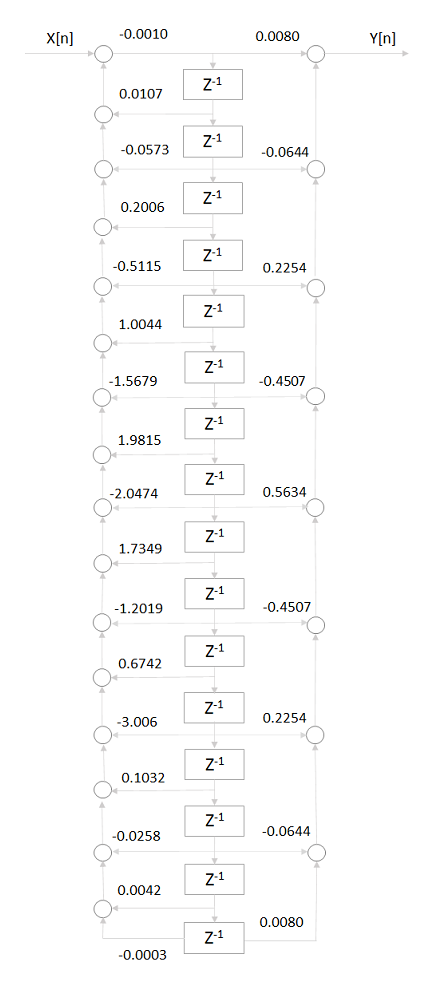
\includegraphics[width=0.6\linewidth]{fir real.png}
    }
    \caption{Direct Form II Block Diagram for Hdiscrete;BSF (z)}
\end{figure}


\newpage

\subsection{FIR BPF Filter Design using Kaiser Window}
Stopband and Passband Tolerance($\delta$) = 0.15\\
Therefore, Kaiser parameters,\\
$\Delta\omega_T$ = $\omega_{s2}$ - $\omega_{p2}$ = $\omega_{p1}$ - $\omega_{s1}$ = 0.03768\\
A = -20$log_{10}$ $\delta$ = 16.4782\\
\begin{equation}
    N_{min} = \lceil\frac{A - 8}{2.285*\Delta\omega_T}\rceil = \lceil\frac{16.4782 - 8}{2.285*0.03768}\rceil = 98.47 
\end{equation}
As A $<$ 21, therefore, shape parameter in Kaiser window, $\alpha = \beta = 0$ (Rectangular Window).\\
The Kaiser window has to operate on ideal BPF filter, which is approximated as a separate function using truncated time domain response of ideal LPF filter. This introduces {\bf non-ideality} which results in {\bf increased order} of Kaiser window than necessary.\\
Therefore, length of Kaiser Window (L) = $N_{min} + 1 + 16$ = 115.47.\\
The transfer function of resultant BPF filter is given by the coefficients mentioned, from zero to increasing time delay (in Z-domain).
\\
\\
fir\_h =


\begin{figure}[H]
    \makebox[\linewidth]{
        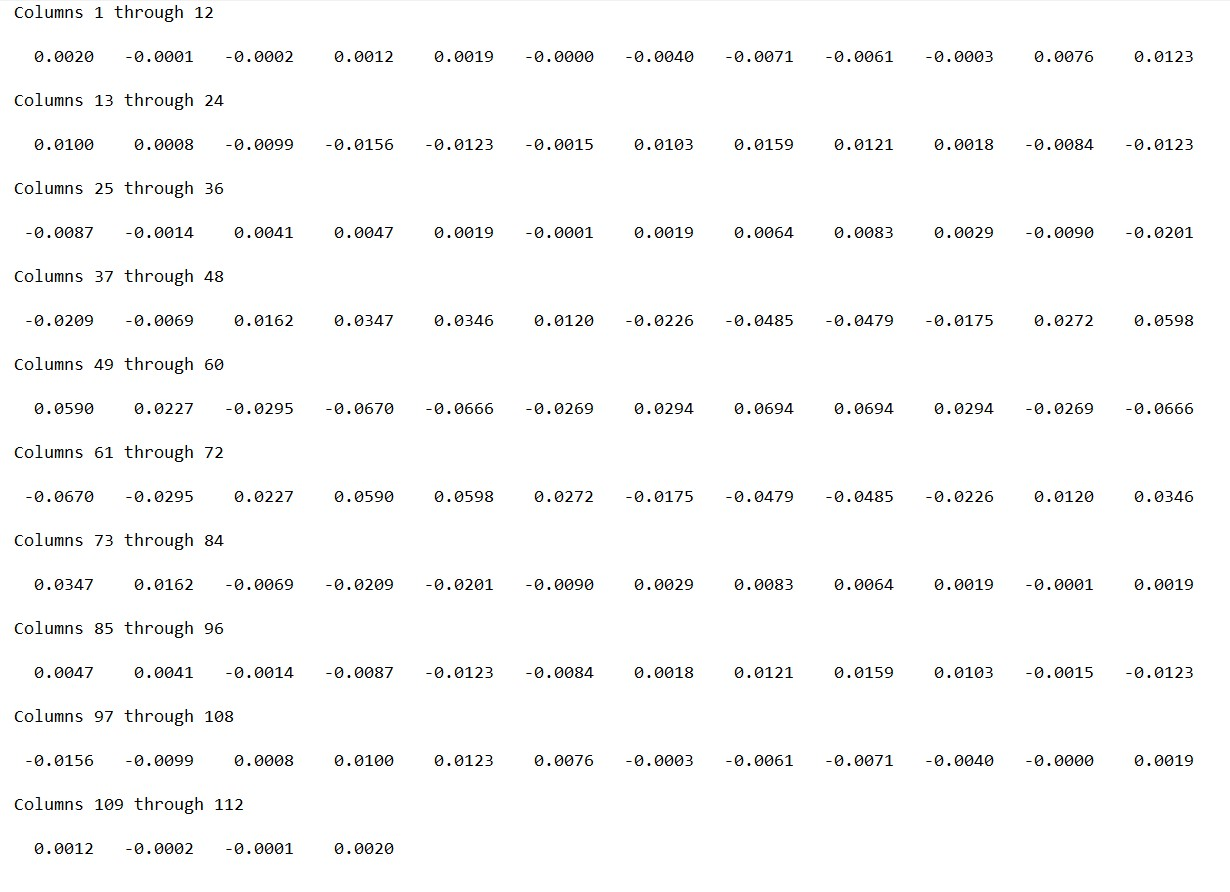
\includegraphics[width=1.3\linewidth]{bpf fir matlab output.jpg}
    }
    \caption{Coefficients of Transfer Function in Z-domain}
\end{figure}

\newpage



\section{Filter - II: Bandstop Filter Design(Chebyschev) }
\subsection{Un-normalized Discrete Time Filter Specifications}
Passband Tolerance = 0.15 (i.e 0.85-1.15)\\
Stopband Tolerance = 0.15 (i.e 0-0.15)\\
Analog Signal frequency range = 140 kHz\\
Sampling Frequency($f_s$) = 250 kHz\\
Transition band on either side of stopband = 2 kHz\\ 
Passband Nature : Equiripple\\
Stopband Nature : Monotonic\\\\
Assigned Filter Number = 46\\
q(46) = 4, r(46) = 46 - 10*4 = 6\\
$B_L(46)$ = 5+ 1.2*4 + 2.5*6 = 24.8 kHz\\
$B_H(46)$ = 24.8 + 6 = 30.8 kHz

\subsection{Normalized Digital Filter Specifications}
Sampling Frequency = 250 kHz\\
Therefore, normalized frequency can be calculated as,
\begin{equation}
    \omega = \frac{\Omega*2\pi}{\Omega_s}
\end{equation} 
Making calculations as per above equation, the modified specifications are,
\\\\
Lower stopband Edge ($\omega_{s1}$) = 0.198$\pi$\\
Upper stopband Edge ($\omega_{s2}$) = 0.246$\pi$\\
Transition band on either side of Passband ($\omega_T$) = 0.016$\pi$ \\
Upper passband Edge ($\omega_{p2}$) = 0.182$\pi$\\
Lower passband Edge ($\omega_{p1}$) = 0.262$\pi$\\
Passband Nature : Equiripple\\
Stopband Nature : Monotonic\\
Passband Tolerance = 0.15 (i.e 0.85-1.00)\\
Stopband Tolerance = 0.15 (i.e 0-0.15)
\subsection{Equivalent Analog filter Specifications}
The analog filter specifications($\Omega$) can be determined using bilinear transformation on normalized specifications($\omega$) as,
\begin{equation}
    \Omega = tan(\frac{\omega}{2})
\end{equation}
Lower Passband Edge ($\Omega_{p1}$) = 293\\
Upper Passband Edge ($\Omega_{p2}$) = 0.436\\
Upper stopband Edge ($\Omega_{s2}$) = 0.321\\
Lower stopband Edge ($\Omega_{s1}$) = 0.406\\
\begin{equation}
    tan(\frac{0}{2}) = 0
\end{equation}
\begin{equation}
    tan(\frac{\pi}{2}) = \infty
\end{equation}
\subsection{Frequency Transformation for BRF to LPF conversion}
The frequency transformation employed for Band stop filter to equivalent low pass filter conversion,
\begin{equation}
    \Omega_L = \frac{B*\Omega}{\Omega_o^2-\Omega^2}
\end{equation}
where,\\ 
B = $\Omega_{p2}-\Omega_{p1}$ = 0.143\\
$\Omega_o^2$ = $\Omega_{p1}*\Omega_{p2}$ = 0.127\\

\subsection{Frequency transformed LPF Specifications}
\begin{equation}
    \Omega_L = \frac{\Omega^2-0.220}{0.154*\Omega}
\end{equation}
Upper Passband Edge ($\Omega_{p1}$) = -0.98\\
Lower Passband Edge ($\Omega_{p2}$) = 1.01\\
Lower stopband Edge ($\Omega_{s2}$) = 0.651\\
Upper stopband Edge ($\Omega_{s1}$) = -0.52\\

Passband Edge ($\Omega_{pl}$) = 1.01\\
Stopband Edge ($\Omega_{sl}$) = min(-0.52,0.65) = 0.52\\
Passband and Stopband Tolerance = 0.15\\
Passband Nature = Equiripple\\
Stopband Nature = Monotonic

\subsection{Analog Lowpass Transfer Function}
The magnitude squared response of the Chebyschev filter in frequency domain,
\begin{equation}
    |H_{analog,LPF}(\Omega)|^2 = \frac{K}{1 + \epsilon^2C_N^2(\frac{\Omega}{\Omega_{pl}})}
\end{equation}
where, K is the normalization constant.\\
Passband Tolerance($\delta_1$) = 0.15\\
Stopband Tolerance($\delta_2$) = 0.15\\
Defining,
\begin{equation}
    D_1 = \frac{1}{(1-\delta_1)^2}-1 = 0.384
\end{equation}
\begin{equation}
    D_2 = \frac{1}{\delta_2^2}-1 = 43.444 
\end{equation}
Taking minimum value of N,
\begin{equation}
    N_{min} = \lceil\frac{cosh^{-1}(\sqrt{D2/D1})}{cosh^{-1}(\Omega_{sl}/\Omega_{pl})}\rceil   = 4
\end{equation}
$\epsilon$ = $\sqrt{D_1}$ =  0.6197\\
Therefore, in s-domain,\\
\begin{equation}
    |H_{analog,LPF}(s)|^2 = \frac{K}{1 + \epsilon^2C_N^2(\frac{s}{j\Omega_{pl}})}
\end{equation}
Solving for the poles of $|H_{analog,LPF}(s)|^2$, we get,
\begin{equation}
    s_k = \Omega_pl sin(A_k)sinh(B) + j\Omega cos(A_k)cosh(B)
\end{equation}
\begin{table}[H]
\centering  % table will be centered.
\begin{tabular}{|c|c|}
\hline  % horizontal line spanning the columns. \\
pole 1($s_{l1}$)	&	 0.123 + j1.397	\\ \hline
pole 2($s_{l2}$)	&	 0.297 + j0.578   \\ \hline
pole 3($s_{l3}$)	&	 0.297 - j0.577   \\ \hline
pole 4($s_{l4}$)	&	 0.123 - j1.396   \\ \hline\hline    % horizontal line.
\end{tabular}
\caption{Table for pole values}
\end{table}
Stable filter implies all poles in left half plane. But there no any poles in left half plane.Hence it is unstable.
\subsection{Analog Transfer Function of BRF Filter}
In $H_{analog,LPF}(s_l)$, substituting,
\begin{equation}
    s_l = \frac{0.143s}{s^2+0.127}
\end{equation}
We get, $H_{analog}(s)$ with mentioned coefficients,\\
Numerator,


\begin{table}[H]
\centering  % table will be centered.
\begin{tabular}{|c|c|c|c|c|}
\hline  % horizontal line spanning the columns. \\
$s^8$ & $s^6$ & $s^4$ & $s^2$ & $s^0$ \\ \hline
1 & 0.5153 & 0.0996 & 0.0085 & 0.0003  \\
\hline    % horizontal line.
\end{tabular}
\caption{}
\end{table}




Denominator,
\begin{table}[H]
\centering  % table will be centered.
\begin{tabular}{|c|c|c|c|c|c|c|c|c|}
\hline  % horizontal line spanning the columns. \\
$s^8$ & $s^7$ & $s^6$ & $s^5$ & $s^4$ & $s^3$ & $s^2$ & $s^1$ & $s^0$ \\ \hline
1 & 0.3752 & 0.6308 & 0.1552 & 0.1311 & 0.0200 & 0.0105 & 0.0008 & 0.0003 \\
\hline    % horizontal line.
\end{tabular}
\caption{}
\end{table}

\newpage
\subsection{Discrete Time Filter Transfer Function}
Analog to discrete time conversion is made using the bilinear transformation,
\begin{equation}
    s = \frac{1-z^{-1}}{1+z^{-1}}
\end{equation}
We get, $H_{discrete,BRF}(z)$ with mentioned coefficients,\\

Numerator,
\begin{table}[H]
\centering  % table will be centered.
\begin{tabular}{|c|c|c|c|c|c|c|c|c|}
\hline  % horizontal line spanning the columns. \\
$z^0$ & $z^{-1}$ & $z^{-2}$ & $z^{-3}$ & $z^{-4}$ & $z^{-5}$ & $z^{-6}$ & $z^{-7}$ & $z^{-8}$ \\ \hline
0.6987 & -4.3141 & 12.7834 & -23.2207 & 28.1357 & -23.2207 & 12.7834 & -4.3141 & 0.6987 \\
\hline    % horizontal line.
\end{tabular}
\caption{}
\end{table}


Denominator,

\begin{table}[H]
\centering  % table will be centered.
\begin{tabular}{|c|c|c|c|c|c|c|c|c|}
\hline  % horizontal line spanning the columns. \\
$z^0$ & $z^{-1}$ & $z^{-2}$ & $z^{-3}$ & $z^{-4}$ & $z^{-5}$ & $z^{-6}$ & $z^{-7}$ & $z^{-8}$ \\ \hline
1.0000  & -5.5926 & 15.0457 & -24.9315 & 27.7116 & -21.1188 & 10.8170 & -3.4267 & 0.5257 \\
\hline    % horizontal line.
\end{tabular}
\caption{}
\end{table}



\subsection{Direct Form II Realization}


\begin{figure}[H]
    \makebox[\linewidth]{
        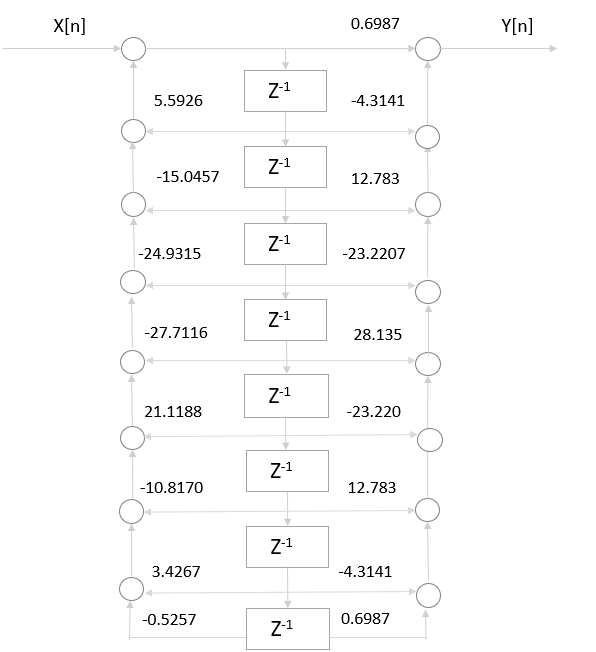
\includegraphics[width=1.1\linewidth]{fir real output.png}
    }
    \caption{}
\end{figure}


\newpage
\subsection{FIR Filter Design using Kaiser Window}
\\ \\ \\
Stopband and Passband Tolerance($\delta$) = 0.15\\
Therefore, Kaiser parameters,\\
$\Delta\omega_T$ = $\omega_{p2}$ - $\omega_{s2}$ = $\omega_{s1}$ - $\omega_{p1}$ = 0.20096\\
A = -20$log_{10}$ $\delta$ = 16.4782\\
\begin{equation}
    N_{min} = \lceil\frac{A - 8}{2.285*\Delta\omega_T}\rceil = \lceil\frac{16.4782 - 8}{2.285*0.20096}\rceil = 19 
\end{equation}
As A $<$ 21, therefore, shape parameter in Kaiser window, $\alpha = \beta = 0$ (Rectangular Window).\\
\newline
\\
The Kaiser window has to operate on ideal BRF filter, which is approximated as a separate function using truncated time domain response of ideal LPF and HPF filter. This introduces {\bf non-ideality} which results in {\bf increased order} of Kaiser window than necessary.\\ \\
Therefore, length of Kaiser Window (L) = $N_{min} + 1 + 12$ = 32.\\ \\
The transfer function of resultant BRF filter is given by the coefficients mentioned, from zero to increasing time delay (in Z-domain).
\\

\begin{figure}[H]
    \makebox[\linewidth]{
        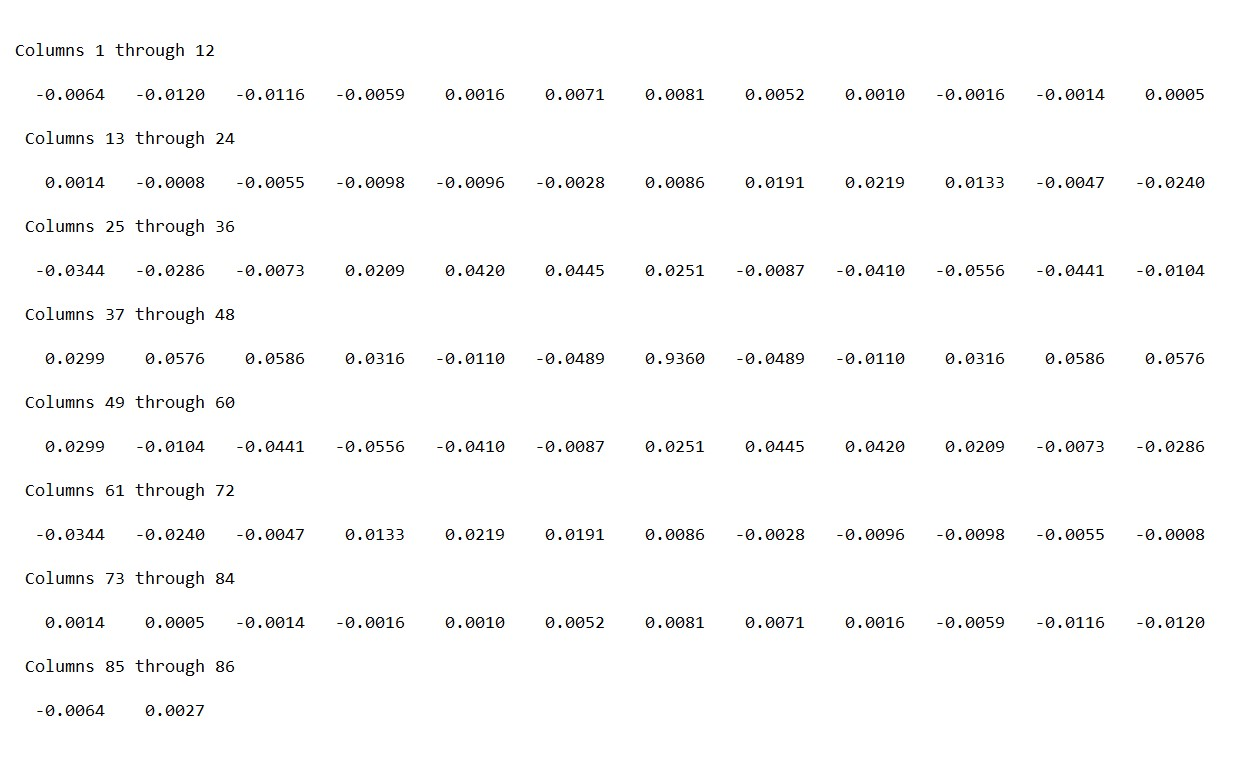
\includegraphics[width=1.3\linewidth]{brf fir matlab output.jpg}
    }
    \caption{Coefficients of Transfer Function in Z-domain}
\end{figure}



\newpage

\section{Matlab Plot}
\subsection{Bandpass Filter (Monotonic)}
\subsubsection{IIR Design}



\begin{figure}[H]
    \makebox[\linewidth]{
        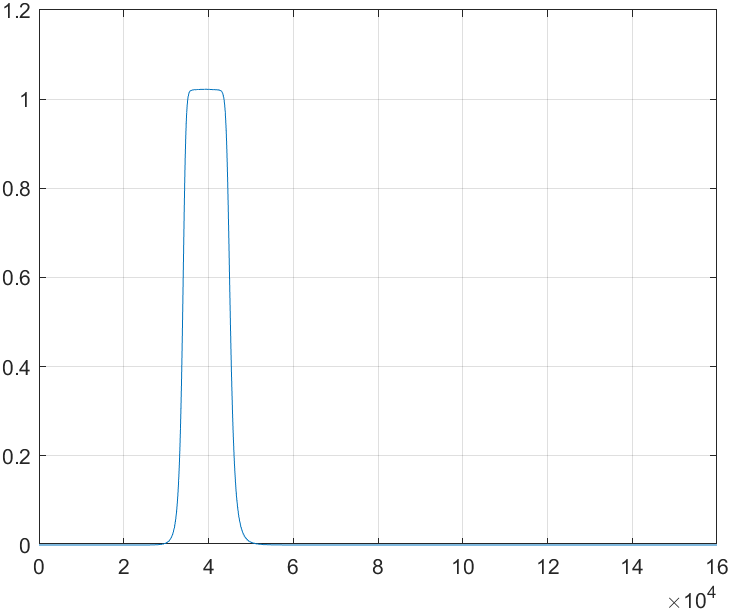
\includegraphics[width=1.3\linewidth]{bpf.png}
    }
    \caption{Magnitude Response}
\end{figure}

\begin{figure}[H]
    \makebox[\linewidth]{
        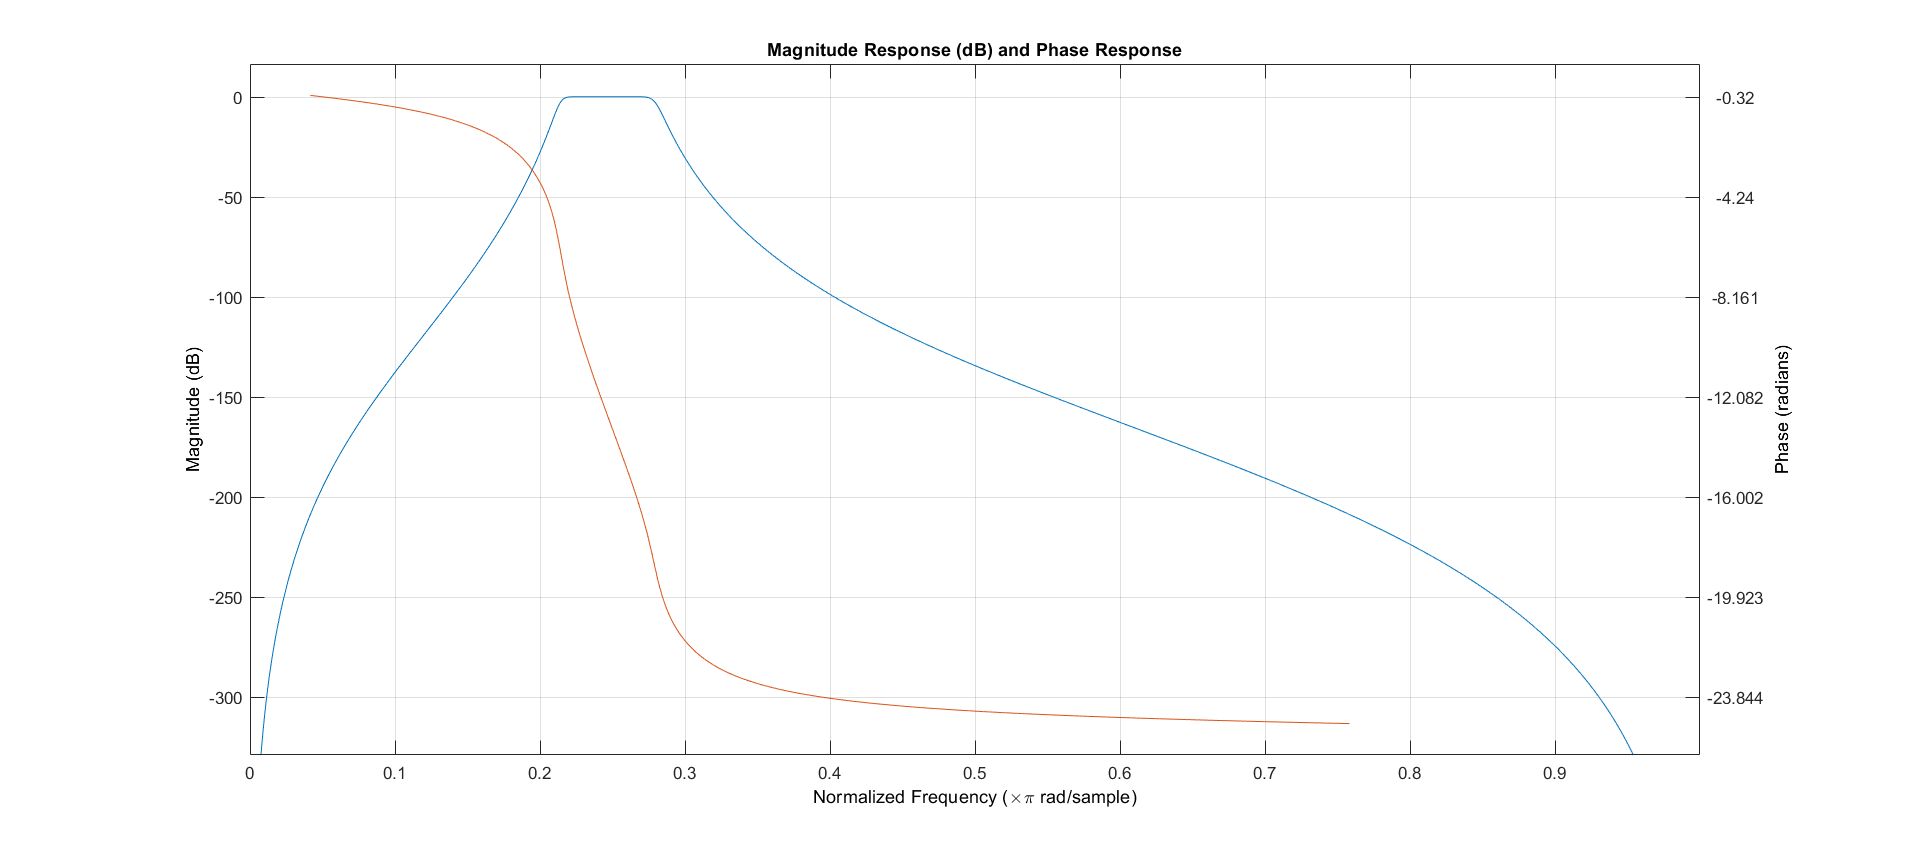
\includegraphics[width=1.75\linewidth]{bpf mag n phase response.png}
    }
    \caption{Attenuation & Phase Response}
\end{figure}


\begin{figure}[H]
    \makebox[\linewidth]{
        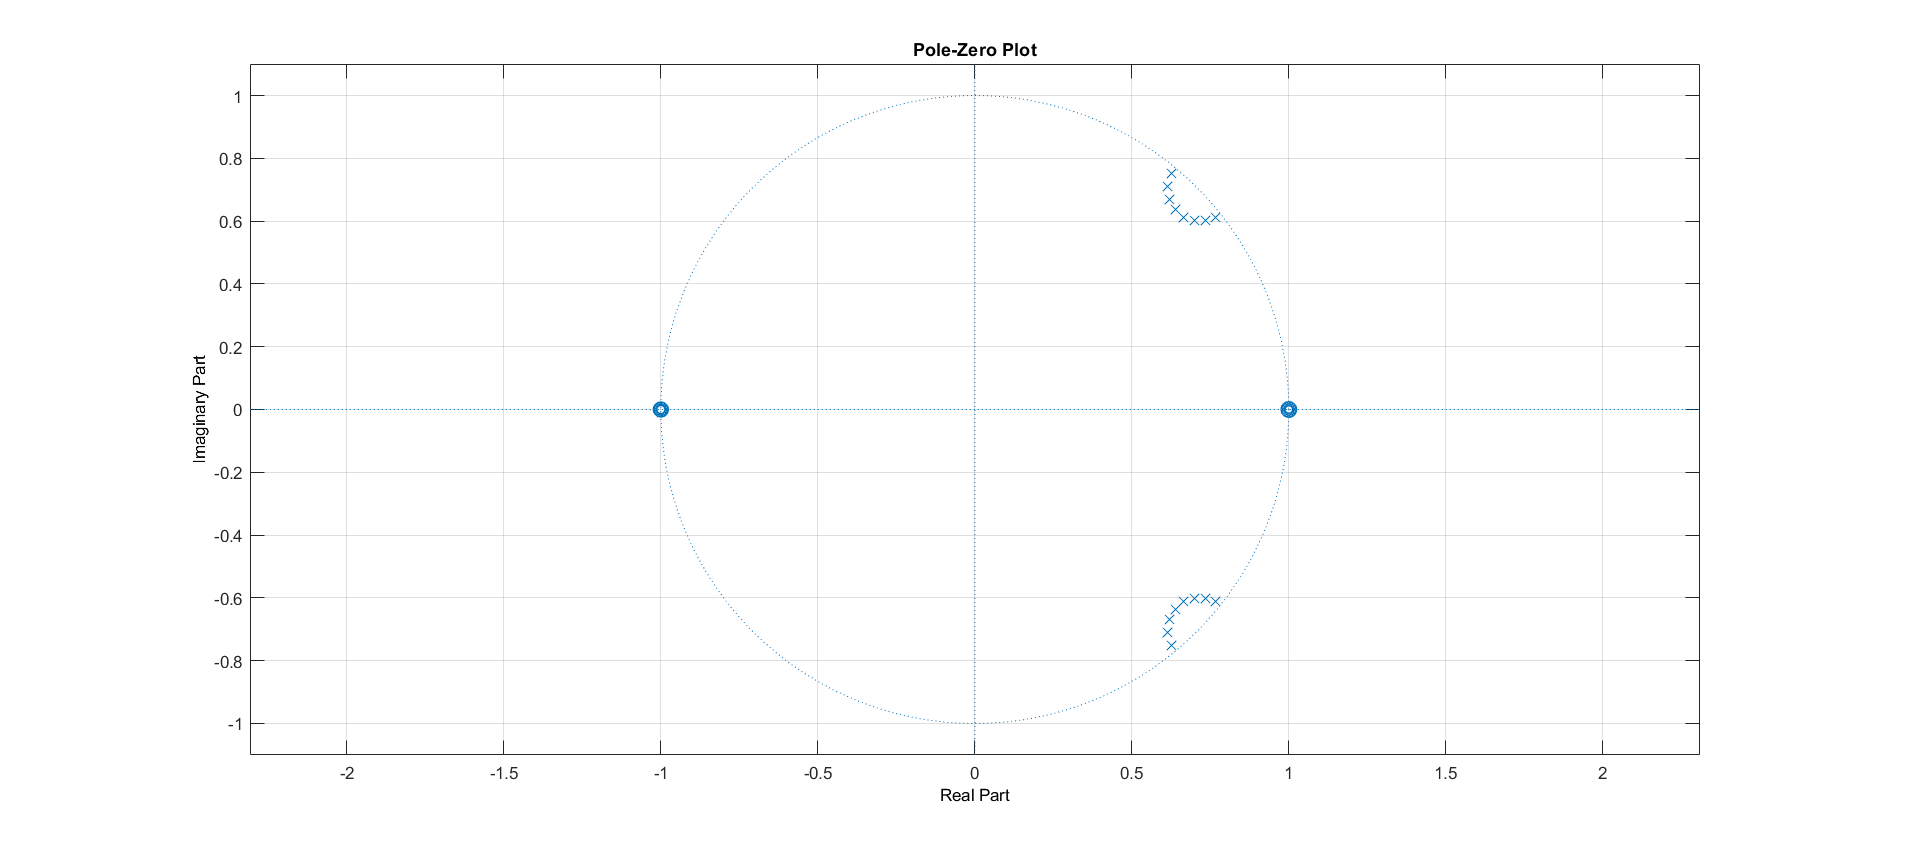
\includegraphics[width=1.75\linewidth]{pole zero plot.png}
    }
    \caption{Pole/Zero Plot}
\end{figure}




The Magnitude plot justifies that the constraints on tolerances are met, the phase plot is non-linear as expected. The pole-zero plot shows all poles(CROSSES) are within the unit circle, hence the filter transfer function is stable.  
\subsubsection{FIR Design}

\begin{figure}[H]
    \makebox[\linewidth]{
        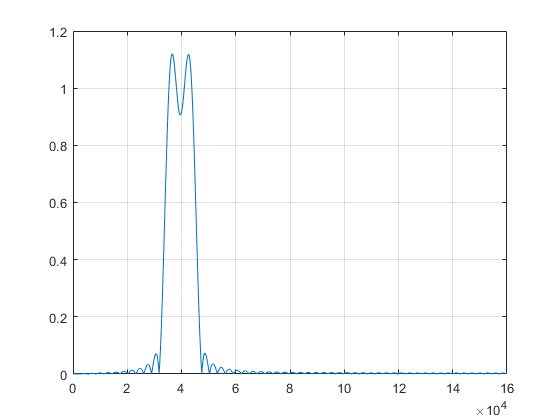
\includegraphics[width=1.3\linewidth]{shabaj.png}
    }
    \caption{Magnitude Response}
\end{figure}

\begin{figure}[H]
    \makebox[\linewidth]{
        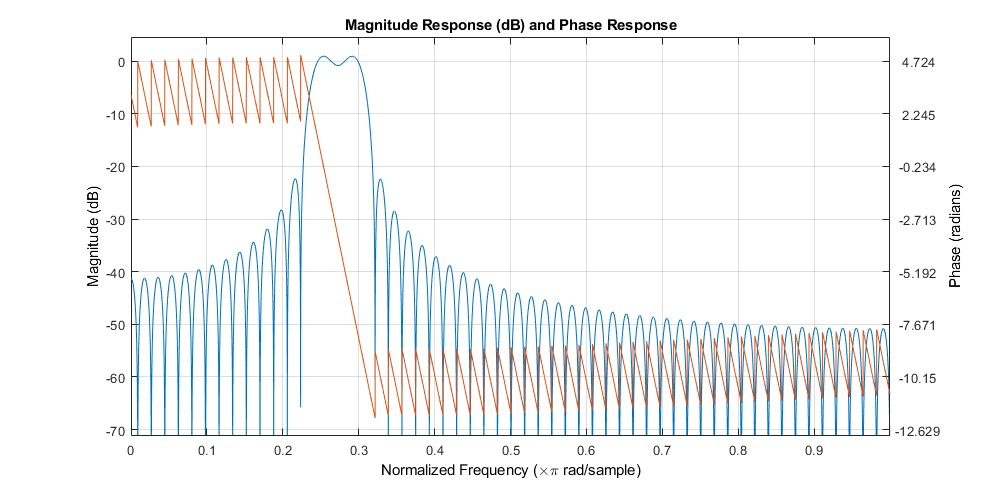
\includegraphics[width=1.6\linewidth]{mag n phase.png}
    }
    \caption{Attenuation and Phase Response}
\end{figure}

The magnitude response plot shows that the constraints on tolerances are met with the phase plot being linear as expected for a FIR filter.

\newpage
\subsection{BandStop Filter (Chebyschev)}
\subsubsection{IIR Design}

\begin{figure}[H]
    \makebox[\linewidth]{
        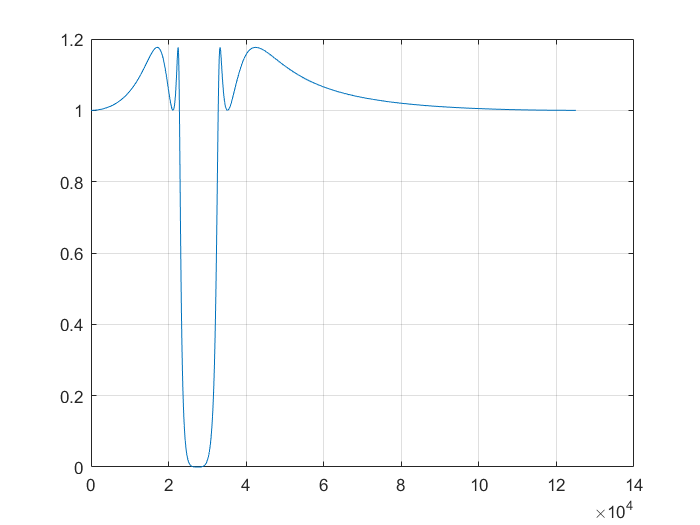
\includegraphics[width=1.3\linewidth]{brf.png}
    }
    \caption{Magnitude Response}
\end{figure}

\begin{figure}[H]
    \makebox[\linewidth]{
        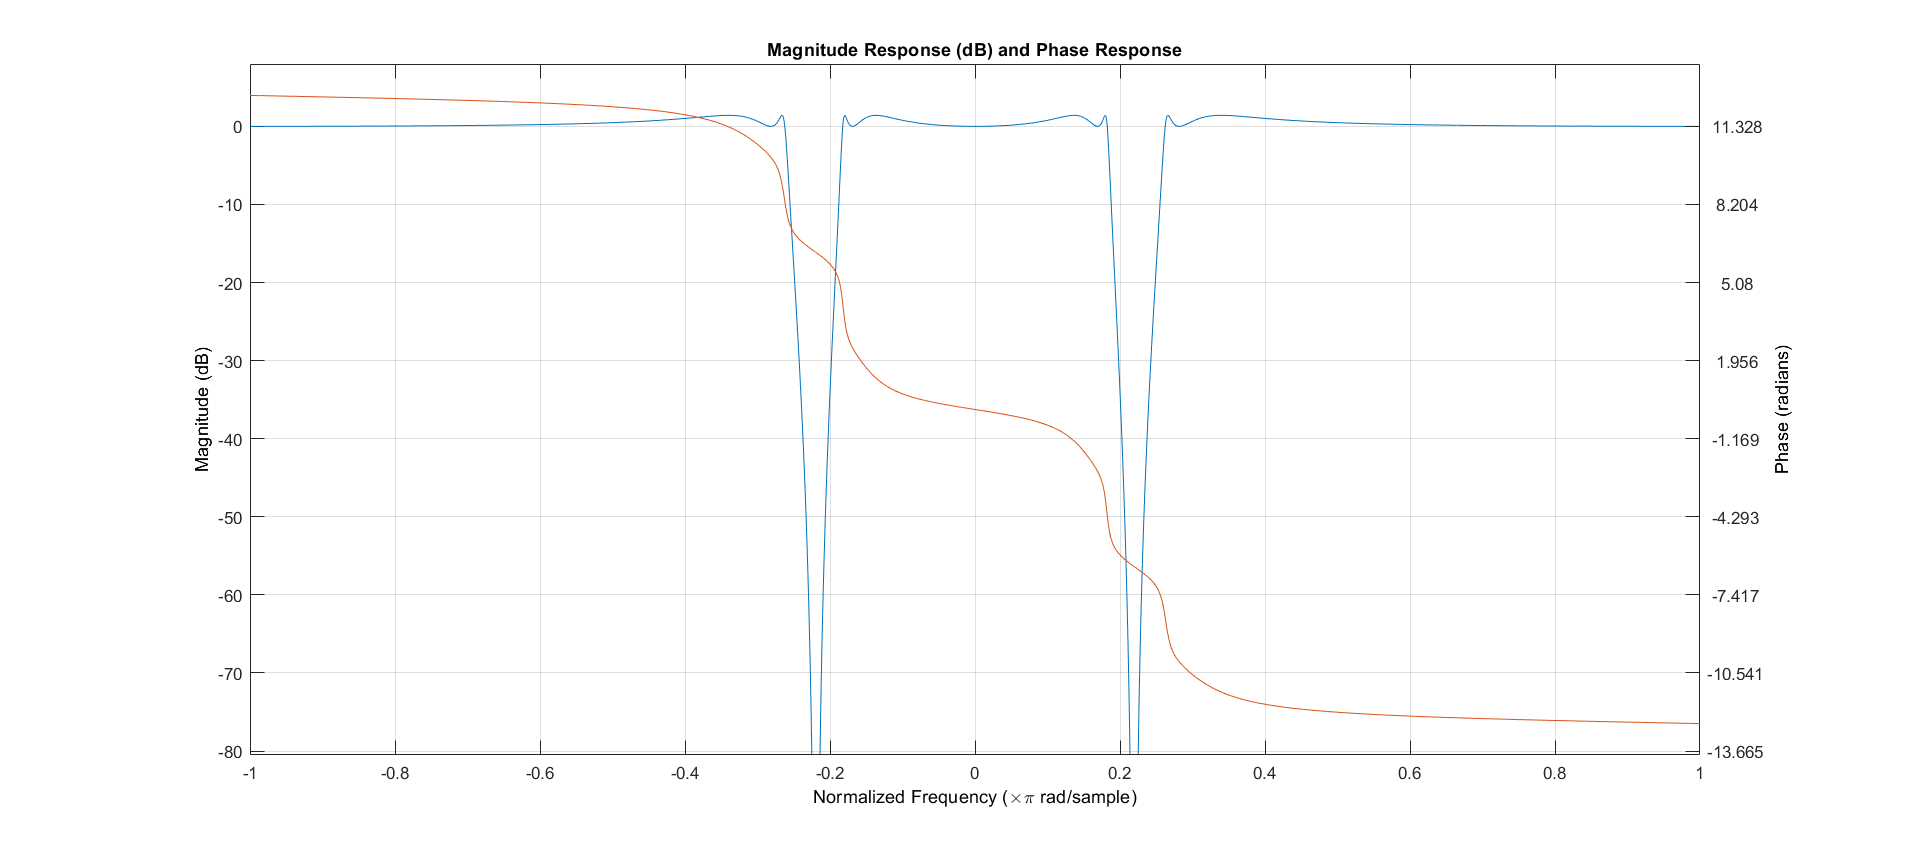
\includegraphics[width=1.7\linewidth]{brf magnitude & phase response.png}
    }
    \caption{Attenuation and Phase Response}
\end{figure}

\begin{figure}[H]
    \makebox[\linewidth]{
        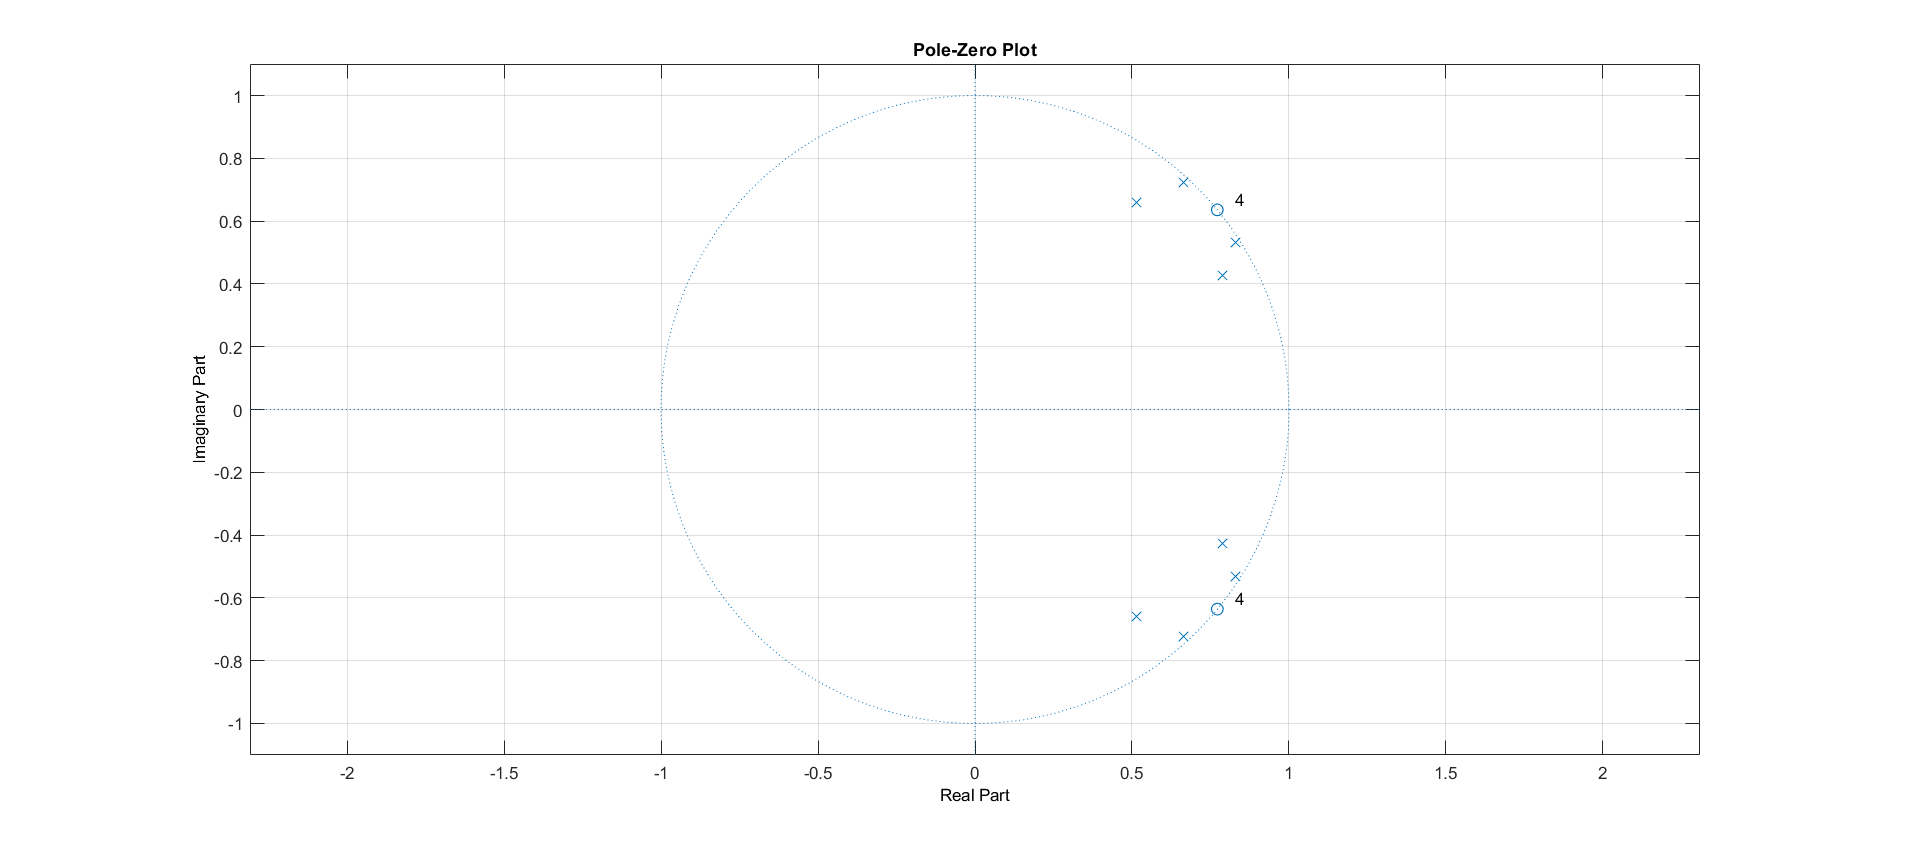
\includegraphics[width=1.7\linewidth]{brf pole plot.png}
    }
    \caption{Pole/Zero Plot}
\end{figure}


The Magnitude plot justifies that the constraints on tolerances are met, the phase plot is non-linear as expected. The pole-zero plot shows all poles(CROSSES) are within the unit circle, hence the filter transfer function is stable.
\subsubsection{FIR Design}

\begin{figure}[H]
    \makebox[\linewidth]{
        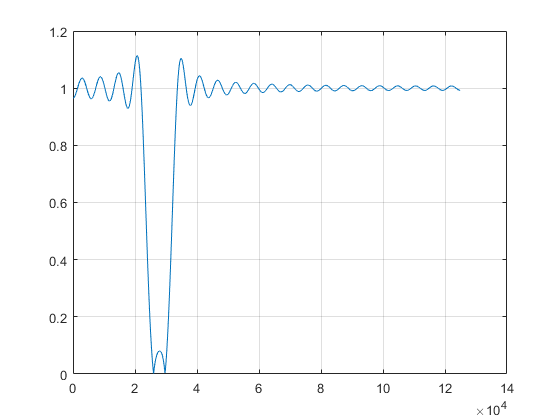
\includegraphics[width=1.3\linewidth]{shabaj22.png}
    }
    \caption{Magnitude Response}
\end{figure}

\begin{figure}[H]
    \makebox[\linewidth]{
        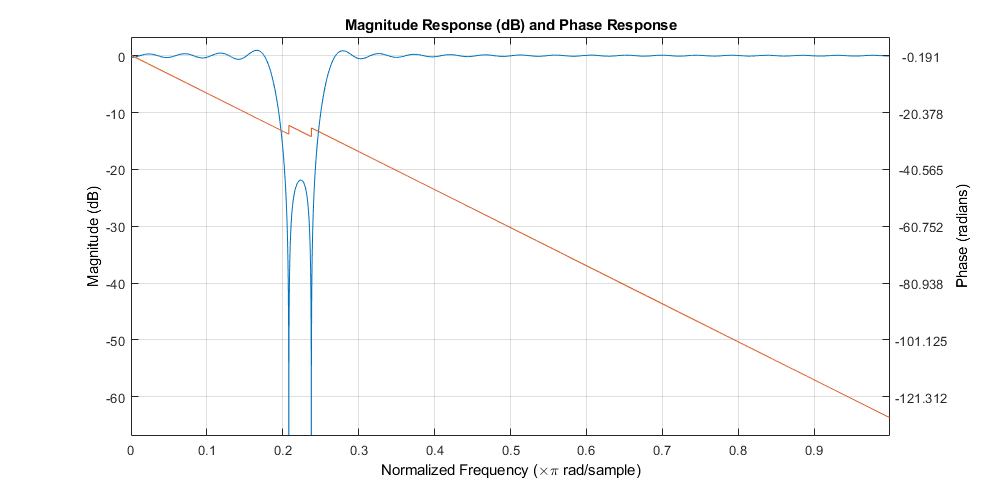
\includegraphics[width=1.6\linewidth]{shabaj brf.png}
    }
    \caption{Attenuation Response}
\end{figure}


The magnitude response plot shows that the constraints on tolerances are met, with the phase plot being linear as expected for a FIR filter.
\end{document}
